\chapter{Implementacja}

\section{Dane wejściowe}
Krok przemiany danych wejściowych do wykorzystania w module został podzielony na dwa osobne etapy. Jeden z tych etapów, nazywany krokiem interpretacji różni się w zależności od źródła skąd pochodzą dane. W zależności od tego, czy system korzysta z danych historycznych w procesie uczenia, czy korzysta z danych aktualnych w celu predykcji inaczej przechodzą proces interpretacji. Drugim etapem jest etap transformacji i wygląda on tak samo dla każdego źródła niezależnie od typu.

\subsection{Interpretacja historyczna}
W przypadku źródła danych historycznych, system musi rozpoznawać epizody działań domowników w celu ich nauki. W tym celu, aby wygenerować zbiór danych uczących, przegląda się posortowaną listę wydarzeń w czasie, celem określenia epizodów akcji. Począwszy od pierwszego wydarzenia w dostępnej dla systemu historii, przegląda się ją w poszukiwaniu ciągu akcji o łącznym czasie nie większym niż pewien z góry określony parametr nazwany \verb+EPISODE_DELTA+ od momentu wystąpienia pierwszej akcji w epizodzie. Ta wartość została wprowadzona w celu sprawdzenia czy zmiana stanu w epizodzie się nie przedawniła. W przypadku gdy jedno urządzenie zmienia swój stan kilkukrotnie w przeciągu jednego epizodu, brana jest tylko pod uwagę policzona zmiana i stan względem poprzedniego, przed liczonym epizodem. W tabeli (\ref{tab:znaleziony_epizod}) został zaznaczony znaleziony dla przykładowej historii epizod. Kolorem został zaznaczony znaleziony przez algorytm epizod akcji. 

Warto zauważyć, że wybrana długość tego parametru będzie mocno wpływała na liczność i wielkość epizodów. Wybranie zbyt krótkiego czasu epizodu będzie rozdzielać powiązane ze sobą czynności ale będzie rozróżniała zmiany stanu tego samego urządzenia w czasie, a wybranie zbyt długiego czasu będzie łączyło kilka niezależnych akcji ze sobą, możliwie je ze sobą niwelując. Sprawia to, że wybranie optymalnej długości epizodu jest bardzo ważne aby system mógł dostosować się do użytkownika.

\begin{table}
    \centering\caption{Tabela przedstawiająca działanie algorytmu szukania epizodów. \label{tab:znaleziony_epizod}}
    \begin{tabular}{|l|l|l|}
        \hline
        Urządzenie              & Stan       & Czas     \dnl
        \dots                   & \dots      & \dots    \nl
        \verb+światło kuchnia+  & \verb+on+  & 16:52:48 \nl 
        \rowcolor{lightgray}
        \verb+światło kuchnia+  & \verb+off+ & 17:32:12 \nl 
        \rowcolor{lightgray}
        \verb+klimatyzacja+     & \verb+17+  & 17:33:00 \nl 
        \rowcolor{lightgray}
        \verb+światło salon+    & \verb+on+  & 17:33:10 \nl
        \rowcolor{lightgray}
        \verb+telewizor salon+  & \verb+on+  & 17:33:15 \nl
        \verb+światło balkon+   & \verb+on+  & 19:32:42 \nl
        \dots                   & \dots      & \dots    \nl
    \end{tabular}
\end{table}

Do określenia działania, dla każdego innego typu urządzeń z osobna, skorzystano z abstrakcyjnej klasy \verb+DeviceHistoryGeneric+, opisujących strukturę funkcji jakie powinna dana klasa implementować w celu poprawnego działania. Abstrakcyjna funkcja na podstawie stanu urządzenia w momencie $t$, stanu urządzenia w momencie $k$ oraz czasu do którego dany epizod powinien się skończyć, zwraca w postaci rzeczywistej liczby, stan oraz przejście stanu dla danego epizodu w czasie. Pseudokod takiej funkcji został zawarty w listingu (\ref{listing:pseudo_get_past_state}). Warto zauważyć, że gdy nie ma poprzedniego stanu, tj. historia nie sięga na tyle wstecz, to kod musi obsługiwać wykrywanie obu wartości. W przypadku interpretacji prostych urządzeń, nie jest to problemem, ponieważ jesteśmy w stanie wydedukować przejście stanu i aktualny stan na podstawie informacji pochodzącej z systemu, tak w przypadku gdy tej możliwości nie ma, pojedynczy błędny wynik powinien być zdecydowaną mniejszością po interpretacji reszty historii.

% todo: zapytać o ten pseudokod
\begin{listing}
\begin{minted}[mathescape]{python}
def get_past_state(aktualny, poprzedni, do_momentu):
    wartość_stanu = 1.0 jeśli aktualny = "on" else 0.0
    # Czy mamy historię na temat poprzedniego?
    jeśli poprzedni nie istnieje:
        wartość_przejścia = 1.0 jeśli aktualny = "on" else -1.0
        return wartość_stanu, wartość_przejścia
    
    wartość_przejścia = 0.0
    # Czy zmiana się nie przedawniła?
    jeśli poprzedni.czas_zmiany < do_momentu:
        wartość_przejścia = 1.0 jeśli aktualny = "on" else -1.0

    return wartość_stanu, wartość_przejścia
\end{minted}
\caption{Pseudokod funkcji interpretującej stany ze źródła historycznego dla typu urządzenia przełącznika astabilnego on/off.} \label{listing:pseudo_get_past_state}
\end{listing}

% Zebrane w ten sposób dane, zbierane są jako listy słowników języka Python w celu łatwiejszego 

\subsection{Interpretacja bieżąca}
Bieżąca interpretacja akcji użytkownika wygląda bardzo podobnie do analizy historycznej. Informacja o bieżącym stanie całego systemu przechowywana jest przez moduł w pamięci. Podczas pracy systemu, mamy pewność, że system AppDaemon zgłosi zmianę stanu tylko jednego urządzenia za każdym uruchomieniem naszej asynchronicznej funkcji. Wiemy zatem, że musimy tylko obsłużyć zmianę stanu jednego urządzenia i zapisać jego stan do pamięci. Informacja o tym, jakie urządzenie zmieniło się do jakiego stanu będzie potrzebna w procesie predykcji, które będzie opisane w późniejszym etapie. Korzystając z tej samej klasy dla typu urządzenia co w przypadku interpretacji historycznej w podobny sposób określamy stan i przejście stanu urządzenia. W tym wypadku ze względu na pewność, że dane urządzenie zmieniło swój stan dokładnie w momencie uruchomienia danej funkcji, obliczanie stanu i przejścia jest zdecydowanie prostsze ponieważ, nie trzeba rozważać przedawnienia się zmiany.

\subsection{Transformacja}
Po prawidłowej ekstrakcji zmian stanu, przed przekazaniem ich do sieci neuronowych dane są dodatkowo przekształcane. W przypadku prostych urządzeń typu przełączniki astabilne, ten proces nie wprowadza do danych żadnej zmiany. W przypadku bardziej skomplikowanych typów danych, takich jak zmienne temporalne wskazujące na np. dzień tygodnia, czy porę dnia, przeprowadzane są pewne dodatkowe operacje rozkładające jedną konkretną informację na kilka różnych wartości, które lepiej będzie sieciom neuronowym powiązać ze akcjami. W celu możliwości wprowadzenia rozszerzalności tutaj ponownie wykorzystano podejście obiektowe i skorzystano z klasy abstrakcyjnej. Zaproponowana klasa abstrakcyjna \verb+Convertable+ opisuje dwie funkcje, które dany konwerter danych musi zaimplementować. Jedna z nich opisuje przejście danych do wersji akceptowalnej przez sieci neuronowe, druga tłumaczy dane wygenerowane przez sieć neuronową do formy obsługiwanej przez resztę systemu. Jednym specjalnym przypadkiem takiego konwertowania danych gdzie potrzebna jest zaimplementowana jedna z obu funkcji, jest przekazywanie zmiennych temporalnych do sieci.

W celu przekazania do sieci jak największej ilości rzeczywiście użytecznych informacji o porze dnia, tak aby była ona w stanie w swojej strukturze zapisać nawyki użytkownika, informacja o czasie jest podzielona. Podział jednej zmiennej czasowej odbywa się poprzez podzielenie jej na 24 różne informacje, gdzie każda z nich wskazuje na pewną wartość zależną od odległości indeksu danej zmiennej od godziny wydarzenia epizodu. Dokładniej, jest to wartość funkcji Gaussa dla wartości zależnej od indeksu, z parametrem $\mu$ ustawionym na moment w ciągu dnia podczas którego wydarzył się ten epizod.

Ważnym parametrem w przypadku funkcji Gaussa poza parametrem $\mu$, jest parametr opisujący szerokość dzwona. W zastosowaniach statystycznych nazywany odchyleniem standardowym $\sigma$. W przypadku takiego zastosowania obliczania wartości funkcji na podstawie czasu, szerokość mówi nam o tym, jak bardzo akcje występujące o konkretnej porze w ciągu dnia mogą być proponowane o innych podobnych godzinach. Ustawienie tego parametru zbyt szeroko, spowoduje że system będzie rozpoznawał wykonywanie konkretnych akcji o bardzo szczegółowych godzinach w ciągu dnia, ustawienie tego za szeroko, będzie proponowało wykonywanie akcji nieadekwatnych do konkretnej pory dnia. Na obrazie (\ref{fig:time_param}) znajduje się przykładowy zarys wartości funkcji dla kilku konkretnych pór dnia, razem z zaznaczonymi dokładnymi przebiegami krzywizny dzwonowej. Każda z zaznaczonych godzin posiada inny parametr $\sigma$ w celu pokazania wpływu tego parametru na policzone wartości.

\begin{figure}
    % todo: wciepać tutaj przykład za szerokiego i za cienkiego ustawienia parametru.
    \centering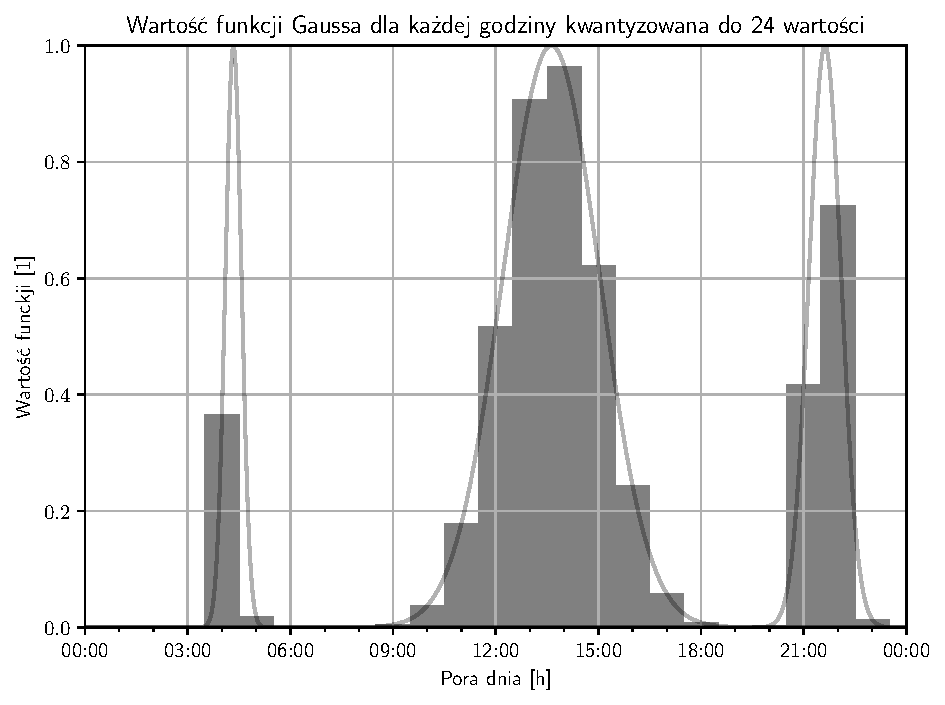
\includegraphics[width=1.00\textwidth]{img/time_param.pdf}
    \caption{Policzone wartości funkcji Gaussa wskazującej czas dla godziny 4:20:02, 13:37:21, 21:37:21.} \label{fig:time_param}
\end{figure}


% Podział jednej zmiennej czasowej na 23 zmienne sygnalizujące porę dnia każda, z nich opisująca jak pora wykonania epizodu jest bliska każdej kolejnej godzinie od 0:00, do godziny 23:00.